\chapter{引言}
\label{cha:intro}
本文提出CloudVision分布式机器视觉云平台,让机器视觉研究人员
可以高效,按需地执行大规模数据的机器视觉任务。本章\ref{sec:background}对论文涉及的
相关领域,包括机器视觉,大数据和云计算进行简单介绍,了解到CloudVision跟
三个领域的关系。
在本章\ref{sec:challenges}描述CloudVision解决的问题与创新点。
最后在本章\ref{sec:main_work}总结主要工作和论文结构。

\section{研究背景}
\label{sec:background}
近年来,机器视觉在各个领域得到广泛的应用,如自动驾驶小车,监控,医疗,交通,IoT,机器人等等。
机器视觉得以蓬勃发展,与大数据和云计算技术息息相关。
新的应用依赖海量数据输入,使用机器视觉算法,同时要求其计算能力随数据的增长而提高。
CloudVision平台使用大数据和云计算领先的方法,提供一个稳定的,针对海量数据的机器视觉执行平台。

机器视觉专门研究怎么用计算机理解可视化的数据,比如使用
从摄影机的图像或者视频,用可视化的数据识别人脸,车或者物体。
最开始机器视觉的研究因为存储和计算能力有限,专注于
小的数据集,比如LeCunn在1989年的神经网络的研究使用了MNIST数据集,
他计算器使用了一个SUN-4/260。\cite{lecun1989backpropagation}
SUN-4/260的CPU是16.67Mhz和最多支持128MB RAM,如果用现在最佳的
机器视觉方法执行在当时的机器,需要执行几年的时间。机器视觉的
一个重要部分是训练数据的大小,如果用更多的数据一般能达到
更好的效果。现在的机器视觉的研究都使用更大的数据集,
另外新的算法对计算能力的要求也增加了,一般要求执行
在大量的CPU和GPU集群。\cite{googlenet2015,baidup2015deepgpu}
在章\ref{subsec:cv_background}我们详细介绍机器视觉的现状。

大数据领域专门研究大数据集如何保存和处理,用处理的数据提供价值。
世界的数据不停的在增长,比如城市里的监控数据,互联网的视频网站。传统
的单处理系统无法保存和处理海量的数据。因此大数据一般分布到集群,然后整个集群
并行处理数据。为了解决机器视觉的海量数据存储和处理问题,可以使用
大数据领域方法。在章\ref{subsec:bigdata_background}我们详细介绍大数据领域的现状。

云计算是一种模式,通过互联网按需提供计算和存储资源。多个用户可以随时随地使用
共享计算资源池(比如服务器,存储,网络,应用,服务)。
为了使得机器视觉能够弹性的处理大数据,可以使用云计算提供灵活的计算基础设施。
在章\ref{subsec:cloud_background}我们详细介绍云计算的模型和现状。




\section{问题与挑战}
\label{sec:challenges}
大数据的技术虽然能改善机器视觉,但是同时也带来新的问题与挑战。
CloudVision想解决的挑战:
\begin{itemize}
  \item 扩展性 \\
        机器视觉最大挑战是扩展性。随着数据的不断增加,系统必须能够弹性地增加存储能力和计算能力,
        从而保证机器视觉算法的可执行性和高效性。与传统的在一台机器上运行机器视觉算法不同,
        将机器视觉运行在集群上,在多个计算节点上并行执行是非常重要的需求。
  \item 基础设施可用性 \\
        基础设施可用性的挑战来自规模和特性。很多大学和研究机构没有大型数据中心专门给研究使用。
        最先进的基于深度学习算法使用大量的CPU或者GPU集群\cite{googlenet2015, google2015rethinking, baidup2015deepgpu}。
        “百度深度学习研究院”用了一个定制的超计算机,里面有34个服务器,每台有两块6核Intel Xeon E5-2620,4个
        Nvidia Tesla K40m GPU,用低延迟的InfiniBand组成一个408个CPU核和136个GPU集群。“Baidu深度学习研究院”基于这个集群,
        通过增加数据训练机器学习的模型,达到了更先进的结果。\cite{baidup2015deepgpu}
        从中可以看出基础设施的重要性,像Baidu这类大型公司,一般拥有大的数据中心和基础设施设计的专家。
        但是大学或者研究机构一般比较缺乏对基础设施的建设。
  \item 并行化 \\
        通过并行化可以解决扩展性的挑战,但是设计并行化的程序也是一个挑战。设计和实现并行化的程序得考虑
        很多方面,包括数据转播,怎么分任务并行执行等等。
  \item 运维负担 \\
        部署,维护和管理需要一定的运维能力和投资。大的集群超过1000个服务器,需要自动化的运维。
        得有运维专家专门运维处理集群,了解具体的软件和基础设施。
  \item 易用性 \\
        目前的主流软件比如OpenCV都需要用户自己安装和部署,解决依赖关系问题等等。这个是一个耗费经历的工作。
        另外如果要在集群上配置OpenCV,其环境的安装和维护将更加复杂。
  \item 可重用性 \\
        机器视觉的研究员经常需在原有的算法做改进或者研究新的算法。他们需要对比新的算法跟目前主流算法的
        准确性,计算时间等等。目前经常需要重新实现原有的算法,浪费大家的时间,因此需要提高可重用性。
  \item 高性能 \\
        高性能挑战主要考虑计算时间和计算的瓶颈,比如集群里的数据传速,硬盘IO等等。
\end{itemize}

\section{相关工作}
\label{sec:related_work}

\subsection{VMX Object Detection/Recognition System}
Vision.ai公司的VMX产品是一个实时的物体检测和分类软件,可以通过Web界面或者RESTful API使用。
VMX提供的物体检测算法专注于速度和准确性,可以快速学习新的模型,将新的模型用来检测,分类,和
跟踪图像或视频里的物体。VMX简单化机器视觉应用在生活中的应用。

\subsection{CloudCV}
CloudCV提供大规模分布式的机器视觉云服务。
CloudCV通过Web界面或者API方式提供最先进的机器视觉算法。整个系统是开源的。\cite{cloudcv2015}

\begin{wrapfigure}{r}{0.50\textwidth}
  \centering
    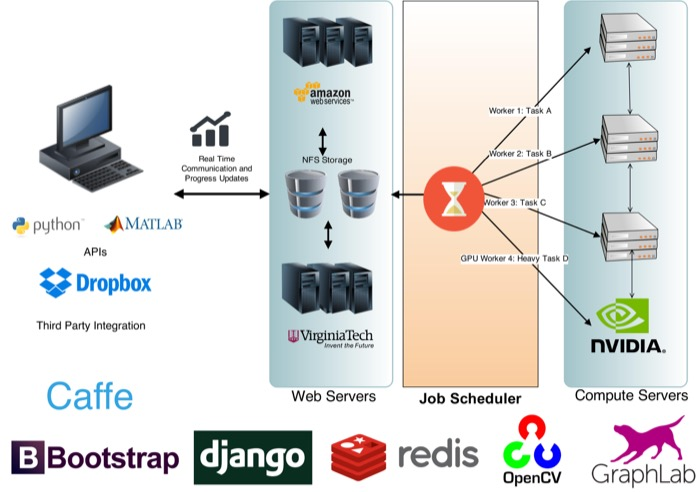
\includegraphics[width=0.49\textwidth]{cloudcv-architecture}
    \caption{CloudCV系统架构。\cite{cloudcv2015}}
  \label{fig:cloudcv-arch}
\end{wrapfigure}
在图\ref{fig:cloudcv-arch}可以看到CloudCV系统的架构。Web Servers基于Django的Web开发框架提供
一个HTTP API和界面。API暴露的接口有:图片分类,DeCAF特征抽取,图像人物识别,
Image Stitcing。数据保存到一个NFS(Linux Network File System)服务器。
在任务调度方面,CloudCV使用Python的Celery框架,为每个节点分配特定的任务。
它们通过不同的队列将任务调度到不同的节点组。按任务类型分队列,这样可以将需要GPU的任务调度
到有GPU的节点。所有计算节点从信息队列中收到需要执行的任务。计算节点使用AWS,Azure和Virginia内部
云平台提供基础设施资源。机器视觉任务主要基于Caffe和OpenCV实现。

\subsection{相关工作结论}
VMX和CloudCV都使得机器视觉的执行更加简单。VMX是一个专有软件,CloudCV是一个开源软件。
两个系统都缺乏一个研究员的场景,允许研究员自己定制算法并大规模执行。CloudCV和VMX主要针对
用一些他们包装好的算法但是没有提供一个可以执行自己的机器视觉应用的平台。另外也没有提供
大数据存储的能力,现实生活中的数据集越来越大,需要一个分布式存储保存。CloudCV用到的NFS无法
扩展到大规模使用。

\section{本文主要工作}
\label{sec:main_work}

本论文工作主要是基于大数据和云计算模型,实现大规模分布式机器视觉执行平台CloudVision。
本节将简单介绍论文三个工作重点:
\begin{itemize}
  \item 大数据,云计算和机器视觉的混合研究

        为了提供一个更好符合现在的研究员的平台,我们
        研究了机器视觉主流方法和实现。目前机器视觉研究面对数据大小和处理需求的增长。其他的研究领域
        解决类似的问题,所以为了不做重复的工作,我们也研究和调研大数据和
        云计算的领域。

  \item CloudVision架构设计与实现

        基于大数据和云计算领先研究,设计CloudVision可扩展的架构。本文章描述
        CloudVision架构的细节和系统的实验方式。

  \item CloudVision平台建设及实验验证

        为了提供一个开发和实验环境,我们建立了清华软件学院的信息系统与工程研究所的私有云。
        实验主要证明架构的选择和扩展性。

\end{itemize}



\chapter{机器视觉,大数据和云计算的现状}
\label{sec:current_state}

\section{机器视觉研究现状}
\label{subsec:cv_background}
互联网公司像Facebook和Google通过文字的数据分析理解用户的兴趣,
和爱好然后用这些信息推更有效的广告,设计新的产品
等等。数据已经开始作为互联网时代的金子。因此通过分析大
量的可视化的数据就可以带来更大的价值。在自主车领域
需要事实分别出来周边的物体,基于周边环境信息做决定,
自主车基于多个头像拍周边的环境。

机器视觉是一个专
注与分析,处理和理解可视化数的数据的领域。可视化的数据
是图片,视频,多生物的数据等等。在最近几年机器视觉的应
用变了更广阔,主流的应用是自主车,车牌监控,机器人,物
体检测。


\subsection{主流作法}
大部分主流的物体检测做法是有一个特征抽取和分类物体过程。\cite{juan2009comparison}
图片原始的信息有每个pixel的颜色度(RGB),这些
原始的信息在多大机器视觉应用场景,无法高效直接在分类器使用。
在机器视觉,特征是为应用场景可以更好描述图片的相关信息。
在本章\ref{intro:image_features}会纤细介绍主流的图片特征。

在分类的过程,首先需要基于机器学习的算法,学出来一个模型,
模型可以当作物体的分类器。
学模型有两个方式,有监督学习和无监督学习。在物体检查和大部分机器视觉应用
分类器使用一个有监督的学习算法。监督学习需要有标的训练数据。
在本章\ref{subsubsec:classifier}会纤细介绍主流的分类器方法。

在图\ref{fig:cloudvision-cvworkflow}可以看到第一步是在训练数据
抽取特征,用特征和标训练出来模型。训练后了模型,可以使用无标的
图片抽取特幀,然后使用学习好的模型分标给图片。
\begin{figure}[H]
  \centering
    \includegraphics[width=0.98\textwidth,trim=1 1 4 1,clip]{cloudvision-cvworkflow}
  \caption{机器视觉主流作法}
  \label{fig:cloudvision-cvworkflow}
\end{figure}

从1989年已经开始有人用神经网络在机器视觉的任务,
Yann Lecun使用了神经网络检测图片里面的数字。\cite{lecun1989backpropagation}
他使用了一个16x16图片输入层每个输入神经对应图片的一个像素点,3个隐藏层,
总共有1256个神经,9760个参数。最后
输出层有10个神经对应每个数字的概率。神经网络的学习需要大量的计算能力,
LeCunn那时候用了3天的时间训练出来参数。考虑到更大的数据集,像素度更高的
图片和更多的隐藏层会发现那个时候计算能力是最有限制。

Lecun做的方法只和是在小的固定的图片。物体识别应用不需要
所有像素点,且更有价值是图片的最有兴趣的点比如物体的边界和特性。
所以从1995到2010主要研究在人工的特征和特征编码与表示。

在1999,Lowe发布了
Object recognition from local scale-invariant features介绍了
SIFT(Scale-invariant feature transform,尺度不变特征转换)。\cite{lowe1999object,lowe2004distinctive}
当时基于SIFT特征可以达到最先进的结果。SIFT主要价值
在于可以从图片只拿到物体上的局部兴趣点,而且这些兴趣点不会被大小和
旋转收到影响。大小和旋转不影响SIFT的特征是在物体检测更重要,因为
经常一个物体在不同的图片有不同的大小和旋转。
光用SIFT对于一些基本的应用很合适但是在物体检测同一类型的物体
会有一定的不同点。光用SIFT就无法抽象出来物体,所以采用了
特征编码和表示。在2004年推出了用BoW在物体检测里面,
抽SIFT特征后用特征编码做出来一个BoW表示描述图片的信息,
用BoW表示当作SVM分类其的输入和训练。\cite{csurka2004visual}
重新达到了最先进的结果。一直到2010大部分研究在于人工特征和特征编码和表示。
在2006发布的Beyond Bags of Features: Spatial Pyramid Matching
for Recognizing Natural Scene Categories,做了BoW和SIFT的改进
达到了新的最先进的结果。 \cite{lazebnik2006beyond}
在本章\ref{subsubsec:image_features}
会详细介绍抽SIFT和相关特征的方法与编码方式比如BoW,VLAD和Fisher Vectors。

从2010开始,深入学习把LeCunn用到的神经网络又复活来了,
主要靠Alex Krizhevsky发布的ImageNet Classification with Deep Convolutional Neural Networks。
这次把神经网络做的更深度和大。打败了当时
所有最先进的研究,包含基于SIFT特征的方法。以来20多年的
计算能力提高和训练数据集大小的曾长,Alex推出一个更深度和大的神经网络。
在图\ref{fig:cnn-architecture}可以看到CNN的深度神经网络
有6000万个参数,65万个神经,5个卷积隐藏层。输出层
有1000个神经,每个神经对应ImageNet的一个物体类别。
跟1989年Lecun的网络对比,参数增加了大概6300倍。
数据集有120万个高请有标识的图片。通过2个GPU并行计算加速了整个训练过程。
最后用了6天训练出来了模型。\cite{krizhevsky2012imagenet,lee2009convolutional}
\begin{figure}[H]
  \centering
    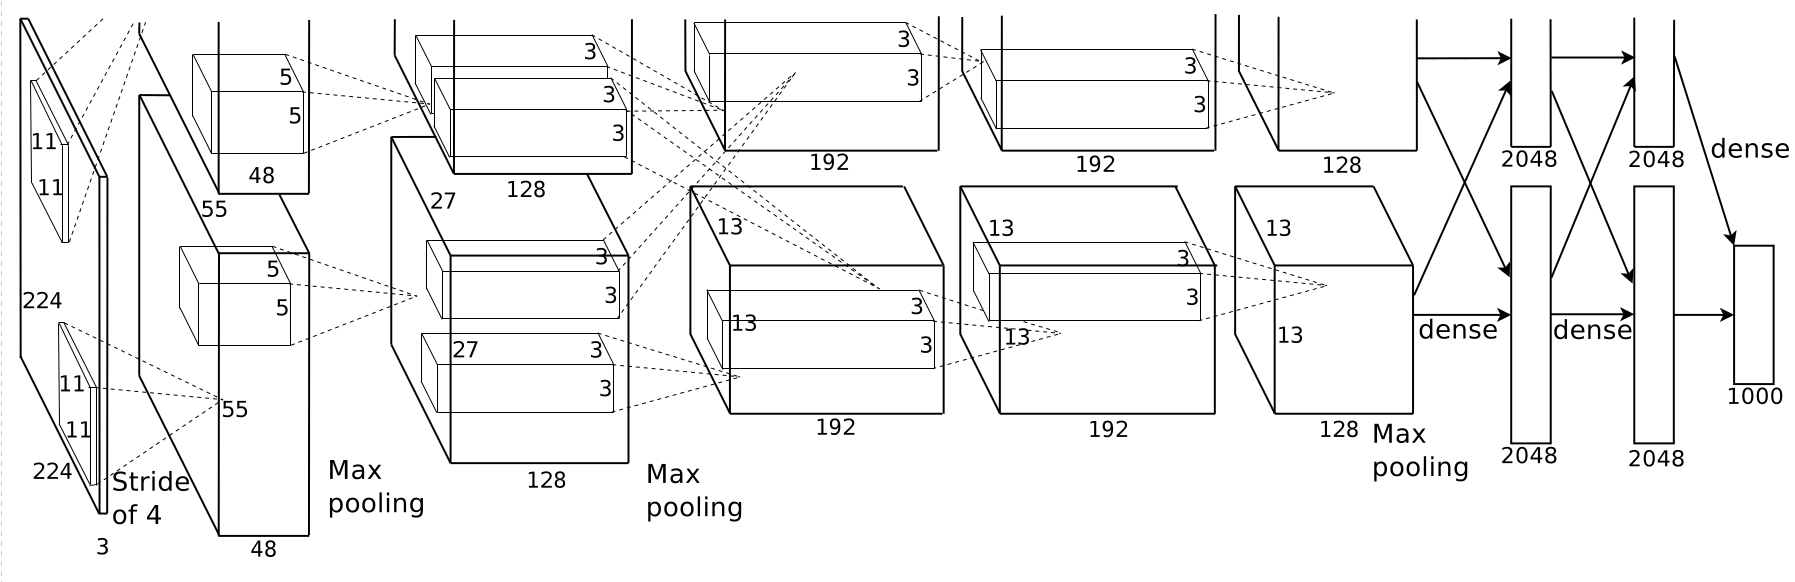
\includegraphics[width=0.98\textwidth]{cnn-architecture}
  \caption{CNN神经网络架构。\cite{krizhevsky2012imagenet}}
  \label{fig:cnn-architecture}
\end{figure}

CNN用同一个网络抽特征和分类物体类型。前面的的层是用来学
特征,然后他最后的输出层作为分类器,训练的时候统一学习整个网络模型。
虽然在CNN网络也可以把分类其与抽特征分开,用输出层前面一层作为一个4096维的Feature 
Vector,叫做CNN特征。然后可以用CNN特征同样用SVM的分类器,去掉了CNN的输出层。
\cite{razavian2014cnn}

现在主流做法多数使用深度学习达到最先进的结果,但是SIFT特征和
特征编码与表示也还是有研究空间和应用。SIFT相关的特征计算快也
不需要一个计算量很大的学习过程。
SVM到现在一直站稳了分类器的优选位子,无论用深度学习
的特征或者SIFT都使用SVM的分类器。

\subsection{常用的特征与特征编码}
\label{intro:image_features}
本章现在常用的特征与表示详细介绍不同特征的特点,抽取方法,缺点与亮点。
最后讲特征的转码与表示方法的特点,转码方法,缺点与两但。
这章把特征分成两种:人工特征与学习出来的特征。人工特征由于人手工制作的抽取
方法,基于有确定性的算法规定怎么抽取特征。学习出来的特征是基于
训练神经网络学出来特征的模型。人工特征有SIFT,SURF,HOG和其他的。
人工特点经常为特定应用场景制作,因此在某个应用能达到最先进的结果
但是无法应用在其他的应用场景。深度学习出来的特征经常可以在不同的
应用场景通用。学习出来的特征需要一个很大的数据集才能达到好的效果。
人工的特征完全不需要训练所以也不以来数据集。学习出来的特征
可以采用别人在数据集已经训练好的模型直接使用。

\subsubsection{人工特征介绍}
人工特征是由于人通过有确定性的算法抽取图片的兴趣点,过滤没有用的信息。
特征的兴趣点可能是边缘,图像梯度大的地方,物体等等。
局部特征是从整个图片先找出关键点然后从关键点抽取特征描述。
全局特征是从整个图片算出特征描述,不需要找出关键点。
生下来我们介绍SIFT的局部特征,因为很多特征是积累SIFT的研究。
最后介绍一个主流的全局特征HOG。

\subsubsection{SIFT特征}
SIFT(Scale-invariant feature transform,尺度不变特征转换)是
一个局部特征描述。\cite{lowe1999object}为了可靠的识别,很重要的是抽取的特征
在图像大小,旋转,噪点和声的变化中,一样可以检测到图像的兴趣点。
这样的点一般在图像的高对比度的区域,比如物体的边缘。
另外一个重要的特点是,兴趣点之间的相对位子信息不影响物体检测。
SIFT主要在物体检测和分类使用。

SIFT的算法分两段:特征关键点检测和特征描述。在特征关键点检测阶段,
SIFT找出所有兴趣点。在特征描述,SIFT从每个关键点抽取一个128维的
向量描述各个关键点。\cite{wiki:sift}
在图\ref{fig:sift-keypoints-localization}可以看到SIFT检测到的
关键点的例子,所有圈子表示一个SIFT的关键点。

\clearpage
\paragraph*{特征关键点检测}
\begin{wrapfigure}{r}{0.33\textwidth}
  \centering
    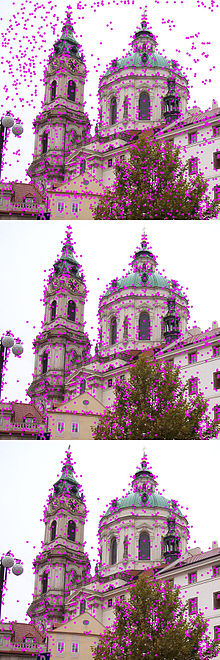
\includegraphics[width=0.32\textwidth]{sift_keypoints_localization}
    \caption{SIFT关键点检测过程。图片源:\cite{wiki:sift}}
  \label{fig:sift-keypoints-localization}
\end{wrapfigure}
SIFT特征关键点提取算法第一步,是为了边缘检测,在多个尺度用高斯滤波器,
提取不同尺度高斯模糊的图像的最大值或者最小值高斯差距。
高斯差DoG定义成$D \left( x, y, \sigma \right)$。
$D \left( x, y, \sigma \right) = L \left( x, y, k_i\sigma \right) - L \left( x, y, k_j\sigma \right)$
,这里$L \left( x, y, k\sigma \right)$是在原生的图像$I \left( x, y \right)$应用了高斯滤波器
$G \left( x, y, k\sigma \right)$,在高斯滤波器$k \sigma$表示尺度,
因此$L \left( x, y, k\sigma \right) = G \left( x, y, k\sigma \right) * I \left( x, y \right)$。
高斯差图像是尺度$k_i\sigma$高斯模糊的图像和尺度$k_j\sigma$的差距。
生产了高斯差图后,关键点是多迟到的高斯差图之间的最大值或者最小值。通过
对比,在高斯差图里的每个像素点跟8个在同一尺度像素点和9个在不同尺度的相应像素点,
算出最大值和最小值。算出来的最大或者最小值作为SIFT选择关键点。这一步,
用高斯滤波器会找出关键点叫做尺度空间极值检测。在图\ref{fig:sift-keypoints-localization}
最上面的图片,可以看到尺度空间极值检测找出的关键点。

通过尺度空间极值检测找到了太多关键点,其中有邻近太近的和不稳定的点。
所以在关键点检测第二步做关键点精确定位,丢弃低对比度的关键点和消除边缘过度的点。

首先通过二次泰勒级数展开高斯差的多尺度空间$D \left( x, y, \sigma \right)$,
做数据的内差,在不同尺度的临近关键点找出极值。
在第一步检测的候选关键点作为泰勒级数的起源。

从泰勒展开的函数取导数,从导数算出极值,然后算候选关键点到极值距离,
如果候选关键点离极值远说明有更好的候选关键点,因此可以消除本候选点。
通过求泰勒展开函数二阶导数,可以过滤掉低对比度的关键点,
如果值小于0.3可以消除候选点。

物体的边缘因为对比度高还是有很多
关键点,目标是在边缘只有几个关键点。为了达到这个效果,
SIFT算出在关键点Hessian矩阵的两个特征值,然后用两个特征值的比值过滤
消除边缘点。在图\ref{fig:sift-keypoints-localization}最下面的图片显示
边缘消除过程的效果

\paragraph*{特征关键点分配方向}
现在所有关键点有尺度不便性,但是我们也希望关键点有旋转不变性。
这一步是基于图像的梯度方向和幅度算出来。这样可以相对于方向
算出来特征描述,达到旋转不变性。
不变性算法如下:每个关键点尺度的周边的像素,使用高斯模糊的图$L \left( x, y, \sigma \right)$,
算出梯度方向和幅度。
算出梯度方向的公式:$$m \left( x, y \right) = \sqrt{\left( L \left( x+1, y \right) - L \left( x-1, y \right) \right)^2 
                  + \left( L \left( x, y+1 \right) - L \left( x, y-1 \right) \right)^2}$$
算出梯度幅度的公式:$$\theta \left( x, y \right) = \mathrm{atan2}\left(L \left( x, y+1 \right) - L \left( x, y-1 \right),
               L \left( x+1, y \right) - L \left( x-1, y \right) \right)$$
\begin{wrapfigure}{r}{0.49\textwidth}
  \centering
    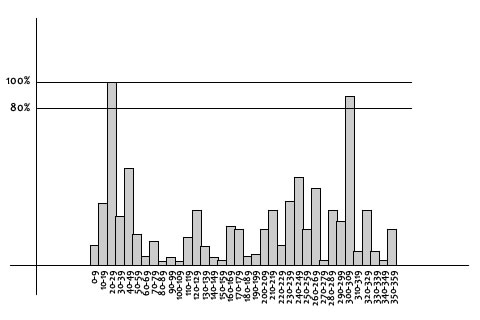
\includegraphics[width=0.48\textwidth]{sift-orientation-histogram}
    \caption{SIFT关键点梯度直方图例子。 \\
             图片源:\cite{aishack:sift-orientation}}
  \label{fig:sift-orientation-histogram}
\end{wrapfigure}
然后用一个直方图统计每个像素点的方向。直方图分成36个方块,
每一个方块表示10度,比如方块1表示所有0-9度的方向像素点,方块2表示
10-19度。那如果周边像素点方向是15度会加入到方块2,
加入的量是根据像素点幅度量添加。
做出来统计所有周边像素点梯度直方图后,可以分配关键点的主要方向和幅度。
所有直方图高峰80\%以内,创建新的在同一尺度和位子的关键点,分配相应的方向。
这个过程可以从一个关键点分成多个不同方向的关键点。
在图\ref{fig:sift-orientation-histogram}的关键点梯度方向直方图的例子,
20-29度的方块 是直方图的高峰,310-319度的方块是在高峰的80\%以内,因此本关键点
会分配20-29度的方向,同时克隆一个新的关键点分配310-319度。

\paragraph*{特征描述}
检测到了图像的关键点和分配了方向后,SIFT可以算出来每个关键点的特征描述向量,
目标是每个关键点有一个极富特色描述,但是为了后续不同图片对比还是够宽容。
SIFT描述向量,可以理解为关键点周围的局部梯度方向的直方图。

\begin{wrapfigure}{r}{0.49\textwidth}
  \centering
    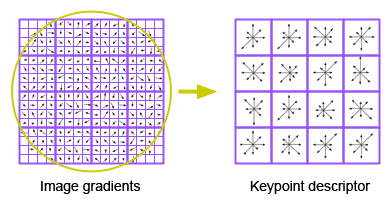
\includegraphics[width=0.48\textwidth]{sift-descriptor}
    \caption{SIFT特征描述。源:Cornell CS664}
  \label{fig:sift-descriptor}
\end{wrapfigure}
SIFT在关键点周边分出一个16x16像素区域,关键点在区域的中心,然后再
把16x16的区域分成16个4x4的区域,可以参考图\ref{fig:sift-descriptor}的
左边的图。在每个4x4的区域算出梯度方向直方图,直方图有8个方块,
每个直方图方块表示$360 / 8 = 45$度,梯度的幅度和离关键点的距离作为
直方图加入的值。因此有16个直方图,每个直方图有8个方块,最终特征描述
是所有规范化直方图的值,造成了一个$16 * 8 = 128$的向量。
在图\ref{fig:sift-descriptor}的右边可以看到描述向量的例子。


\subsubsection{其他局部特征}
SIFT的成功发起了很多新的基于SIFT的特征的研究。在几年内
出了新的人工的局部特征:PCA-SIFT,SURF,FAST,BRIEF,ORB。
\cite{ke2004pca, bay2006surf, fast2006machine, calonder2010brief, rublee2011orb}
新的局部特征主要贡献点在于速度,可以更快的抽取特征,降低计算时间,因为
SIFT无法满足实时的要求。\cite{juan2009comparison, calonder2010brief}

PCA-SIFT的贡献点在于SIFT特征描述的优化,提供一个更有独特性,
更好处理图像变形和更紧凑的描述特征向量。通过实验发现PCA-SIFT
的特征描述跟其他图片特征描述对比(feature matching)运行时间
比原生的SIFT快。\cite{ke2004pca}
PCA-SIFT算法跟SIFT算法区别在特征描述的算法:SIFT使用
在关键点的周边的16x16像素点区域,PCA-SIFT用一个
41x41像素点区域。SIFT把这个区域分成8个4x4区域算出梯度直方图,
作为SIFT的128维的特征描述向量。
PCA-SIFT把41x41的区域分成用2个39x39区域,
算出横向梯度直方图和纵向梯度直方图,然后做Principal Component
Analysis降低唯独算出一个36维的特征描述响亮。
在后续研究对比了PCA-SIFT的特征发现它在描述独特性比SIFT
和其他特征差。\cite{mikolajczyk2005performance}

SURF的主要贡献点在于优化整个关键点测和特征描述的过程,做法也是被SIFT启发的。
SURF的作者说SURF运行时间快几倍,另外在不同图像变换可以更稳定检测到关键点。\cite{bay2006surf}
SIFT检测过程用多个尺度的图像算出高斯差图金字塔,在金字塔找出极值作为候选关键点。
SURF关键点检测过程,先计算积分图,然后用Hessian矩阵的行列式找出局部变化
最大的点作为候选关键点。
SURF特征描述在每个关键点,基于积分图快速计算Haar特征的总和作为
特征描述向量。

\clearpage
\begin{wrapfigure}{r}{0.49\textwidth}
  \centering
    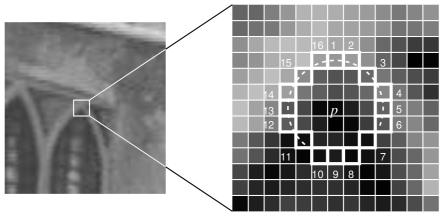
\includegraphics[width=0.48\textwidth]{fast_detector}
    \caption{FAST检测角点做法。\cite{fast2006machine}}
  \label{fig:fast-detector}
\end{wrapfigure}

FAST是一个角检测算法,没有提供描述子。
主要贡献点在于快,作者提到在实时处理视频,
SIFT和SURF都不能及时处理完视频的帧。SIFT
使用DoG(高斯差图)检测关键点,FAST提到了
一个新的方式可以检测到关键点。
FAST在每个图像像素点通过本点周边的像素点直接检查是否是一角点。
具体被检测的像素点,划分一个16个像素点的卷,然后通过16个点的不同
像素密度判断是否是角点。在图\ref{fig:fast-detector}可以看到
怎么划分16个像素点的卷。为了提高检测角点的正确率,FAST算法
用机器学习的决策树分类器。

BRIEF是一个特征描述子,没有包含关键点检测。\cite{calonder2010brief}
主要贡献点在于一个更小的用二进制表示特征描述响亮,可以
用快的Hamming距离做特征对比不同图像的BRIEF特征描述。
BRIEF描述法是在关键点取出一个模糊$S \times S$的Image Patch $p$。
BRIEF的binary test function $t$,是在Patch内的像素点对比像素密度分配boolean值:
$$
t(p; x, y) = \begin{cases} 
      1 & if p(x) < p(y) \\
      0 & else 
 \end{cases}
$$
这里$p(x)$是像素点$x$在模糊的patch $p$的像素密度。选择$n_d$个$(x, y)$
对作为BRIEF的$n_d$长度的特征描述。作者推荐$n_d$使用128, 256, 512,太小了
会影响特征描述的独特性,但是太大了对存储和计算需求有影响。

ORB是一个基于FAST角点检测器和BRIEF特征描述子的特征,
重点是提供一个效果跟SIFT一样但是可以实时计算的特征。
主要贡献是提供旋转不变性和提高图像噪点抵抗性,原生的
FAST和BRIEF都却的。ORB推出了oFAST(Orientated FAST),
先创建一个多尺度的图像金字塔,在每个金字塔的level用FAST
检测关键点然后,按Harris的corner measure顺序选前$n$个关键点。
通过多尺度金字塔可以提供尺度不变性。在每个检测到关键点
ORB使用Intensity Centroid算出方向。
另外ORB推出了rBRIEF特征描述,是一个旋转不变的BRIEF。ORB
先旋转image patch然后再算出BRIEF特征描述。作者通过实验发现
旋转的BRIEF特征描述的反差比原生BRIEF大,影响特征描述的独特性。
通过一个自己的算法ORB学习怎么更好的选无相关的$(x, y)$对做
binary test,这样降低旋转BRIEF的方差。


\subsubsection{全局特征 - HoG}
全局特征从整个图像算出特征描述,不需要一个特征关键点检测的过程。
在2005年,N. Dalal和B. Triggs推出了HoG(Histogram of Gradients)
方向梯度直方图。\cite{dalal2005histograms}
当时用在图像的人类识别,检测图像哪里有人类。另外的应用场景包括
物体识别,场景识别和视频里的人类识别。HoG也是收一个被SIFT
启发的特征。

\begin{wrapfigure}{r}{0.49\textwidth}
  \centering
    \captionsetup{justification=centering}
    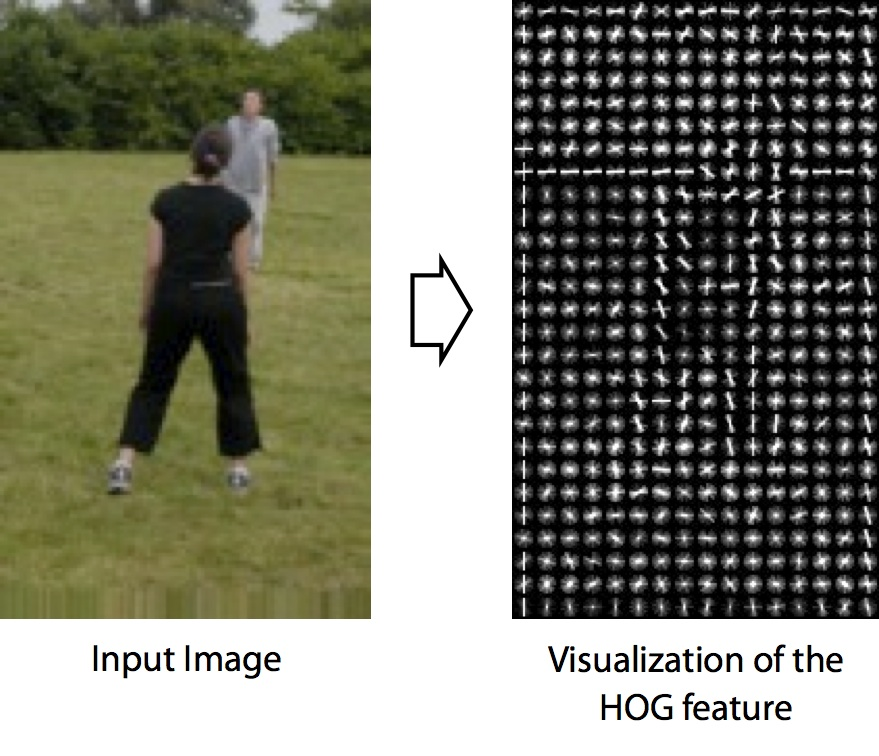
\includegraphics[width=0.48\textwidth]{hog-visualization}
    \caption{可视化HOG的特征描述。\\
             源:Cornell CS4670}
  \label{fig:hog-visualization}
\end{wrapfigure}
HoG的算法把整个图像分成$n$个连在一起的区域(cells),每个区域先单独算出来
它的梯度方向与梯度直方图。为了考虑照明和对比度的变化,HoG把多个区域
连在一起然后归一化。所有区域归一化后的直方图作为HoG的特征描述响亮。
在图\ref{fig:hog-visualization}可以看到图像到HoG特征的可视化。

在论文里面用了SVM分类器,用HoG的特征描述向量输入到SVM。
作者在MIT pedestrian database训练了和测试了HoG + SVM的
人类识别性能,几乎能正确识别整个测试数据集。因此作者
再做了一个新的更有挑战和大的人类识别数据集。


\subsubsection{深度学习特征}
深度学习特征用机器学习的算法自动学出来图像的特征抽取与表示方法。
在人脸识别,物体识别还有其他场景,学习出来的特征获得了现在先进的结果。
\cite{taigman2014deepface, krizhevsky2012imagenet}
在2014年,Razavian研究了用CNN作为特征在其他应用场景,对比CNN和基于SIFT
的效果。在它测试数据集和应用场景,基于CNN的特征的效果,都比基于人工特征的方法好。
\cite{razavian2014cnn}

%Deep Learning Features, mainly explain CNN and how we can use it as feature.
%R-CNN, SPP, Fast R-CNN, Faster R-CNN, CDBN(Convolutional Deep Belief Network)

%Edge Detection
%DeepEdge, DeepCountour


\subsection{特征转码与图像表示}
\label{subsubsec:feature-encoding}
在图\ref{fig:image-representation}可以看到经典的工作流。
第一步从图片抽取特征描述比如SIFT,
第二部从特征描述转码到图像表示(Image Representation),
然后图像表示用于在分类器的训练和分类。
特征转码用一个词典(Visual Codebook)分配每个特征描述行属于
哪个词,总结这个信息作出一个图像表示响亮。
使用特征编码与图像表示,可以帮助提高识别类型的通用性。比如需要分类器
在鉴于,影像,灯光和闭塞变化中,还是能识别出属于同一个类型。
最早的方法是在2004年发布的Visual Categorization with Bag of Keypoints,
应用了Bag-of-Words的模型在机器视觉的任务。\cite{csurka2004visual}
后续基于BoW改进的方式包含 Fisher Vector转码和VLAD。
\cite{perronnin2007fisher,jegou2010vlad}本章先介绍BoW理解转码和词典生产的过程,
然后介绍Fisher Vector和VLAD怎么改进BoW。
\begin{figure}
  \centering
    \includegraphics[width=0.98\textwidth]{image-representation}
    \caption{特征转码到图像表示的过程。}
  \label{fig:image-representation}
\end{figure}

%Bow Intro, Dictionary Generation, Encoding, Classifier example

\subsection{数据集}
为了让研究员能够重现和对比结果,机器视觉领域提出不同应用场景的标准化的数据集。
这些数据集,是为具体应用场景标识好的数据,提供一个训练数据集,和测试数据集。
常用的分类数据集包括:
\begin{itemize}
  \item ImageNet - 是一个不停增长的分类检测和物体定位数据集,每个类别平均有500多个图像。
        ImageNet目前最大和常用的分类数据集。ImageNet 2014分类数据集有120万的图像。\cite{deng2009imagenet}
  \item Pascal VOC(Visual Object Classes) - 是一个分类和检测数据集。\cite{everingham2010pascal}
  \item Caltech 256 - 是一个256类别的分类数据集,总共有30607个图像。数据来源是Google Images。\cite{griffin2007caltech}
\end{itemize}
        


\subsection{分类器和机器学习}
\label{subsubsec:classifier}
机器视觉应用的最后一步需要做决策,比如识别的应用得决策看到的特征属于那个类别。
这一步,一般使用监督机器学习的方法和训练数据集学出来一个模型,将模型在无知的数据做决策。
机器视觉最经常用到的监督机器学习算法是SVM。

\subsection{相关的软件}
机器视觉软件简化机器视觉的应用开发和研究,主流
的开源软件如下:
\begin{itemize}
  \item OpenCV - 是最丰富机器视觉的库,提供目前主流的人工特征算法,机器学习算法,图像处理功能和人脸识别应用。OpenCV
        主要提供C++接口,另外也有C++ wrappers提供其他语言的接口包括Python,Java和Matlab。
  \item VLFeat - 是一个专注于机器视觉人工特征和特征表示的库。为了提高性能底层是用C写的但是也提供Matlab的接口。
  \item scikit-image - 是一个图像处理和人工特征的Python库。
  \item Caffe - 是机器视觉专注于深度学习的库。Caffe限于单个节点使用,但是可以并行在单个节点的多个GPU。
  \item TensorFlow - 是一个机器智能库,目前专注于深度学习。最新的0.8版本支持在多个节点,多个GPU并行执行。
\end{itemize}



\section{大数据与分布数处理研究现状}
\label{subsec:bigdata_background}
数据增长从稀缺到过多,带来新的好处,但是同时也带来新的挑战。
互联网公司一直跟数据的快速曾长在战斗。谷歌(Google)每天处理24PB的数据。
Facebook的用户每小时保存1000万个图片,每天用户点赞30亿次。点赞的数据
可以用来分析用户的兴趣和爱好,推出更有效的广告。
除了互联网公司之外,其他行业也面对数据成倍曾长的情况,同样想抓我新的机会。
沃尔玛公司(Wal-Mart Stores Inc.),来自与美国是一个在全球运营超市连锁企业,
每小时处理100万的交易,保存到一个超过2.5PB的数据库,从这些数据沃尔玛找出买家的模式。
数据在各个行业变了一个很重要的无形资产。\cite{mayer2013bigdata}

大数据领域属于所有数据超过传统存储容量和处理能力,利用这些海量数据
得到商务的优势。可以用3V数据曾长模型描述数据:
\begin{itemize}
  \item Volume(数据量): 数据的大小比如1PB。
  \item Velocity(速):数据的输入和输出速度,比如每分钟保存1TB新数据。
  \item Variety(多样性):数据包含不同的数据类型,比如文本,视频,图像,社交网络等等。
\end{itemize}
Gartner用3V模型定义成大数据:"大数据是量特别大,高速曾长,多样性的数据
,这些数据为了创造价值需要特殊的技术与分析模型。"\cite{bigdatadefinition}

在2004年Google发布了"MapReduce:简单化集群的数据处理",描述Google内部用的
模型和技术解决大数据的挑战。\cite{dean2008mapreduce}
MapReduce是一个框架,用来在集群并行处理大数据。MapReduce程序组成一个Map(映射)函数和
Reduce(归纳)函数。Map函数一般用来过滤和数据预处理,然后由Reduce函数总结数据比如算出平均值。
用MapReduce函数是一个从函数变成范式借过来的。MapReduce贡献点是在于提出怎么在集群里高效与可靠
并行执行MapReduce程序。MapReduce使用数据的局部性,处理数据在接近的节点减少数据移动。

在2006年Doug Cutting被Google FileSystem和MapReduce收到启发开发了开源的Apache Hadoop。
\cite{gfs2003, dean2008mapreduce, wiki:hadoop}Apache Hadoop是一个开源框架提供
,在普通硬件上的大数据集分布式存储与处理。Hadoop变了一个世界上的大数据技术标准,
大互联网公司和企业都在用,典型的包含Facebook,Baidu,Yahoo,Ebay,Spotify。
在本章\ref{subsubsec:hadoop}会详细介绍Hadoop的框架和架构。

在2009年,UC Berkeley的AMPLab开始开发了Spark,一个开源集群分布式处理框架。\cite{wiki:spark}
Spark改善了MapReduce分布式框架,用内存运算技术提高性能,另外提供一个更灵活
的编程范式,不限于用Map/Reduce函数。Spark编程范式,合适于机器学习的算法和其他
迭代形式的算法。在本章\ref{subsubsec:spark}会详细介绍Spark。



\subsection{Apache Hadoop}
\label{subsubsec:hadoop}
Apache Hadoop是一个开源被Apache维护的分布式存储与处理框架。
Hadoop所有模块都设计到,如果任意件硬件所发生故障不影响数据丢失
和处理的结果。
Apache Hadoop框架核心模块有:
\begin{itemize}
  \item Hadoop Common:所有模块用的程序库和工具。
  \item Hadoop Distributed File System(HDFS):分布式存储文件系统,使用普通的电脑与服务器提供
        高效,容量大的可靠的存储集群。
  \item Hadoop MapReduce:一个基于Google提出的MapReduce范式分布式处理实现集群分布式处理。
  \item Hadoop YARN:集群资源管理,用来调度用户提交的分布式处理任务,比如调度MapReduce任务。
\end{itemize}
除了Apache Hadoop核心之外,Hadoop也变成了一个生态系统,HBase(基于HDFS的NoSQL),Hive(数据仓库)等等都属于
Hadoop的生态系统。Apache Hadoop大部分代码用Java写的,少部分脚本用Python写的,还有少部分Native代码用C写的。

\subsubsection{Hadoop Distributed File System}
\label{subsubsec:hdfs}
HDFS是Hadoop实现的分布式,可扩展,高可用文件系统。一个HDFS集群分两种主要节点:Namenode和Datanode。
HDFS集群一般有一个Namenode,由它保存记录和目录的层次和namespace(命名空间)。Namenode使用inodes表示文件和目录。Inode记录
文件和目录的属性比如权限,修改与访问时间,空间配额和命名空间。HDFS把文件的内容分成多个blocks(块),默认一块是128MB,
然后将每个块独立复制到多个(默认是3个)不同的datanodes。Namenode维护一个命名空间对应块的树,记录文件所有块保存在
那个datanode。

在图\ref{fig:hdfs-arch}描述HDFS的集群架构,为简单起见当时集群保存了一个350MB的文件,名字是example.txt。
文件会分成$\ceil{\frac{350}{128}} = 3$个块,分别为B1,B2,B3。每一块需要保存3份到不同的datanode。

\begin{figure}
  \centering
    \includegraphics[width=0.85\textwidth]{hdfs-arch}
    \caption{HDFS的集群架构。}
  \label{fig:hdfs-arch}
\end{figure}

除了HDFS之外也有其他分布式文件系统可以替代HDFS,这些系统叫HCFS(Hadoop Compatible FileSystem)。
HCFS的文件系统需要实现Hadoop定义的FileSystem API,常用的例子包括用Amazon的S3对象存储替代HDFS。
这样Map/Reduce或者Spark不需要部署HDFS。


\subsubsection{Hadoop MapReduce}
Hadoop MapReduce是Hadoop的分布式处理系统,用户用MapReduce编程模型写程序,
并行执行在Hadoop集群。MapReduce程序有一个Map函数做数据预处理和过滤,另外有一个Reduce函数
提供数据总计。Hadoop MapReduce系统负责调度MapReduce任务,让任务并行的高可用执行在集群里。

Hadoop MapReduce的调度利用到HDFS的数据局部性,任务尽量执行在HDFS的datanode,只处理本地datanode的数据,
这样减少数据转播的开销。MapReduce的实现方法如下:
\begin{enumerate}
  \item 执行Map:每个处理节点使在本地数据上执行用户提供的Map函数,将Map结果保存到处理节点本地的零时存储。
  \item 分布(Shuffle):处理节点按Map结果的Key重新分布数据到所有处理节点。
  \item 执行Reduce:每个处理节点在按Key分布好的本地数据上执行用户提供的Reduce函数。
\end{enumerate}

\subsection{Apache Spark}
\label{subsubsec:spark}
Apache Spark是另外一个Hadoop生态系统的分布式处理系统,替代Hadoop MapReduce。
Spark解决Hadoop MapReduce的限制,第一MapReduce的编程模型不够灵活,第二MapReduce把
中间结果保存到磁盘造成性能问题。

Spark核心贡献点提出了RDD(Resilient Distributed Dataset),一个只读数据结构分布到
集群各个节点的内存。在RDD数据结构上除了Map和Reduce用户可以用其他的函数比如forloop
实现分布式处理,给用户带来更好的编程灵活性,因此Spark合适写迭代算法比如机器学习算法。

\begin{wrapfigure}{r}{0.45\textwidth}
  \centering
    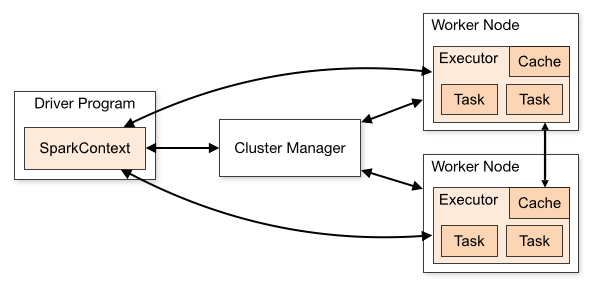
\includegraphics[width=0.44\textwidth]{spark-arch}
    \caption{Spark集群的架构。源:\cite{spark_arch_doc}}
  \label{fig:spark-arch}
\end{wrapfigure}
在图\ref{fig:spark-arch}可以看到Spark的架构。用户写的Spark程序
会执行在一个节点,这个Spark程序叫Driver Program。Driver Program
核心是SparkContext,由SparkContext负责从Cluster Manager申请集群
里的资源,将ClusterManager分配并且执行Spark的executors。SparkContext根据
用户写的程序分配任务(Task)到每个executor,
executors的Task是最终处理数据。如果任务失败了,SparkContext负责
重新调度和分配这个task到executor,提供任务执行的可靠性。
Spark支持多种Cluster Manager,Spark自带,
Apache Mesos和Apache YARN。另外Spark的RDD记录所有操作,如果
保存RDD的划分节点发生故障,Spark会通过操作记录重新计算发生故障的划分。


\subsection{Apache Mesos}
Apache Mesos是一个开源的集群管理软件。Mesos自己定为成
数据中心的内核,抽象集群里计算器的CPU,内存和存储,
让用户容易开发和执行弹性和可靠的分布式系统。

Mesos集群架构分成Mesos Master和Mesos Slave。
Mesos Masters管理所有的slaves。Mesos Frameworks比如Spark,
会从Master收到集群里的资源情况信息,叫Resource Offers,
由于Framework的Scheduler决定要用哪些节点的资源。
如果觉得在资源$X$执行,Mesos Master将Framework的executor
执行在资源$X$。

除了Spark之外Mesos也支持其他软件执行在Mesos集群上,比如Storm,
Marathon,Cassandra,Jenkins。另外用户可以用Mesos的API开发
新的Mesos Framework支持其他的软件。



\section{云计算领域研究现状}
\label{subsec:cloud_background}
云计算是一个通过网络按需求提供计算资源(比如服务器,网络,存储,应用,服务)的模型,
资源可以快速调配和解放,
调配与解放资源需要运营商少量的管理工作。\cite{mell2011nist}
云计算的模型有五个特性:
\begin{itemize}
  \item 按需的自助服务 - 
        用户随时可以调配与使用资源。调配过程不需要任何人的参与。
  \item 用网络提供接入 - 
        资源与功能可以通过网络被访问。推动不同的客户端都可以访问,比如手机,浏览器。
  \item 资源池化 - 
        运营商的的计算资源是池化,动态按需给用户分配物理或者虚拟计算资源。用户无感知
        具体那些物理资源分配给他,用户只知道给他分配了他需要的资源。池化资源例子包括
        存储,计算,内存和网络带宽。
  \item 高弹性 - 
        资源与功能可以弹性的调配与解放。某些场景也提供自动调配与解放支持按业务量的自动扩展。
        对于用户来说,他感知云提供的资源是无限,无论什么时候都可以调配他需要的资源。
  \item 计量服务 - 
        云平台用计量的功能自动控制与优化资源。所有资源的使用的数据报给运营商和用户。
\end{itemize}
云的模型分成不同的服务类型:Software as a Service(SaaS),Platform as a Service(PaaS),
Infrastructure as a Service。SaaS直接给用户提供应用层的服务,用户可以通过瘦客户端使用应用,
用户不需要管理底层的云基础设施。PaaS提供给用户一个软件执行环境,用户可以容易部署自己开发的
或者现有的软件,运营商提供变成语言执行环境,编程库,和工具,用户不需要管理底层的基础设施。
IaaS是提供基础设施的资源比如服务器,存储和网络的资源。
如果用户或者企业想用到云,他可以选不同的云部署模型:
\begin{itemize}
  \item Private Cloud(私有云)- 
        云平台基础设施资源限于单个机构使用。
  \item Public Cloud(公有云)- 
        云平台基础设施资源开放给大家使用。多个用户共享同一个云平台。
  \item Hybrid Cloud(混合云)-
        云平台基础设施是由于公有云和私有云组建的。使用特殊的技术做
        多云平台数据转播和负载均衡。
\end{itemize}

分析了云计算的定义与概念后,可以了解到,它对于用户带来的价值。
通过云提供的按需自助服务,用户自己不需要管理基础资源,他需要资源
可以灵活的占用需要的资源,通过云的多租户性其他用户可以使用他解放的资源,提供
资源的有效使用和快速上线业务能力。

企业可以用云平台减少资本支出,之前企业需要自己长期投资数据中心,用云企业可以
按需求用IT的资源,只付企业用具体用到的资源。

\subsection{Amazon AWS}
Amazon AWS(Amazon Web Services)是美国亚马逊公司提供的公有云。
AWS在12个地区的数据中心,是世界规模和用户最大的公有云。
亚马逊本身是一个电子商务互联网公司,
因此有大量的数据中心投入和IT资源管理的需求。自己要求
所有IT资源是标准化和自动化。算出来发现如果只是自己用
浪费很多数据中心的资源,同时可以当作一个额外的收入。
在2015的第四节,报道的收入是24亿,说明AWS当时的决策
是正确的。

AWS主要提供IaaS服务,计算,网络和存储。计算服务有
Amazon Elastic Compute Cloud(EC2)是基于Xen虚拟化按用户需求
提供虚拟机的计算服务。EC2把虚拟机叫做Instance(实例)。用户
可以随时创建,启动和删除实例,EC2会按照按小时算出用户花的钱。
创建时候可以选镜像和实例类型(Instance Type)。
镜像可以是EC2提供制作好的镜像或者提供自己的镜像。
实例类型定义虚拟机CPU,内存,磁盘或者其他特性比如GPU,SSD。
cg1.4xlarge和g2.2xlarge类型提供NVIDIA Tesla GPU,合适于在
GPU计算应用使用,比如深度学习。

AWS的主要基础设施存储服务有两种,Elastic Block Storage(EBS)和Simple Storage Service(S3)。
EBS给EC2的实例提供块存储,可以理解为虚拟硬盘。EC2实例可以按需求连接和卸载EBS提供的块设备。
S3是一个独立的对象存储服务,可以通过标准的HTTP REST,SOAP,BitTorrent接口,保存,访问,删除任何文件。
S3通过SLA保证数据容量扩展性,高可用和数据持久性。
S3经典用户有Reddit,Dropbox,Tumblr,Pinterest。\cite{wiki:s3}

AWS的基础设施网络有,Virtual Private Cloud(VPC),Elastic Load Balancing(ELB),Route 53。
VPC给EC2的实例内部隔离网络的功能,用户可以按需求定义多个隔离的网络。原来所有EC2的
实例共享一个网络而且所有实例有个互联网IP地址。通过VPC可以提高安全,只对外提供
服务实例分配互联网IP地址,其他使用VPC的网络。另外用户也可以通过VPN,连到VPC内
的实例,这样可以把企业内部数据中心安全的连到VPC内的资源。
ELB是AWS的负载均衡服务,可以把从外面进来的流量均衡到EC2的实例。
提高应用级别的高可用和扩展性。AWS保证负载均衡器本身的高可用与扩展性。
ELB也集成EC2的Auto Scaling功能,压力大时候可以自动扩展添加更多的EC2实例。
Route 53是AWS的高可用和可扩展的DNS服务。Route 53集成AWS的其他的服务,比如
ELB,S3,EC2实力等等。可以用Route 53提供负载均衡的域名。

除了IaaS的基础设施之外AWS也提供一些PaaS服务,其中有
Database as a Service(数据库服务)和Elastic Map Reduce(Hadoop服务)。


\subsection{OpenStack}
\label{subsubsec:openstack}
OpenStack是一个开源软件云平台,主要用于提供IaaS的基础设施服务。
OpenStack由多个组管理数据中心的计算,存储和网络资源池。用户
可以通过RESTful API或者Web UI使用OpenStack的服务。
\begin{wrapfigure}{r}{0.45\textwidth}
  \centering
    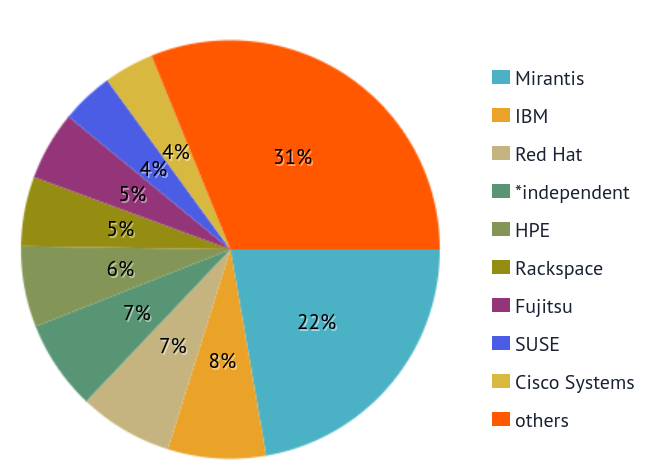
\includegraphics[width=0.44\textwidth]{openstack-mitaka-loc-contributors}
    \caption{OpenStack的Mitaka版本贡献者排名,按Lines of Code排序。\cite{stackalytics_mitaka_loc}}
  \label{fig:openstack-contributors}
\end{wrapfigure}
OpenStack的API抽象出来IT的资源,OpenStack的灵活架构支持多种
技术实现计算,网络和存储的管理。比如计算服务可以用KVM,VMware或者
裸服务器提供给用户计算资源。

OpenStack最早来自NASA和RackSpace合作,开发一个AWS的开源实现。
经过OpenStack的发展和成功,NASA和RackSpace给了非盈利的OpenStack Foundation
所有运营权经营权和所有权,促进开放。


在2016年发布的Mitaka版本,OpenStack由25000贡献者来自1500多不同的公司贡献了OpenStack社区的代码。\cite{stackalytics_mitaka_loc}
在图\ref{fig:openstack-contributors},可以看到全世界前10名公司的贡献者,第一名是Mirantis,第二名是IBM,
第三名是HP和Red Hat(红帽)。多个大企业的贡献和投资意即OpenStack成为开源云平台的标准。

OpenStack在各个行业都有大户包括互联网,金融,电信,教育,企业和运营商。
大部分用户用来内部的私有云,但是也有公司基于OpenStack提供公有云的业务。
在2016的4月OpenStack Foundation做的用户调查,用户提到选OpenStack的主要原因是:
\begin{itemize}
  \item 标准化开放平台的API,统一在公有云和私有云可以通用。
  \item 通过开放的平台避免厂家锁定,提供可选的技术方案。
  \item 通过快速上线新应用,提高创业性和竞争能力。
  \item 提高运营效率。
  \item 减少成本,OpenStack比其他私有云方案成本底。
  \item 参与活跃全球性的技术社区,吸引技术人才。
  \item 用可控制的平台达到安全和隐私的目标。
\end{itemize}
CERN是一个大的OpenStack用户,有15,000多个物理服务器和100PB数据量的集群通过OpenStack
提供给CERN的研究员IT资源。CERN的Large Hadron Collider记录粒子碰撞粒子的数据,每次碰撞
的数据量是1PB左右,然后需要处理集群分析并保存数据。通过OpenStack,研究员于自助的方式
使用IT的资源,同时CERN的IT部门可以更高效的运营数据中心的资源。\cite{cern_user_story}

\paragraph{OpenStack架构}
\begin{figure}
  \centering
    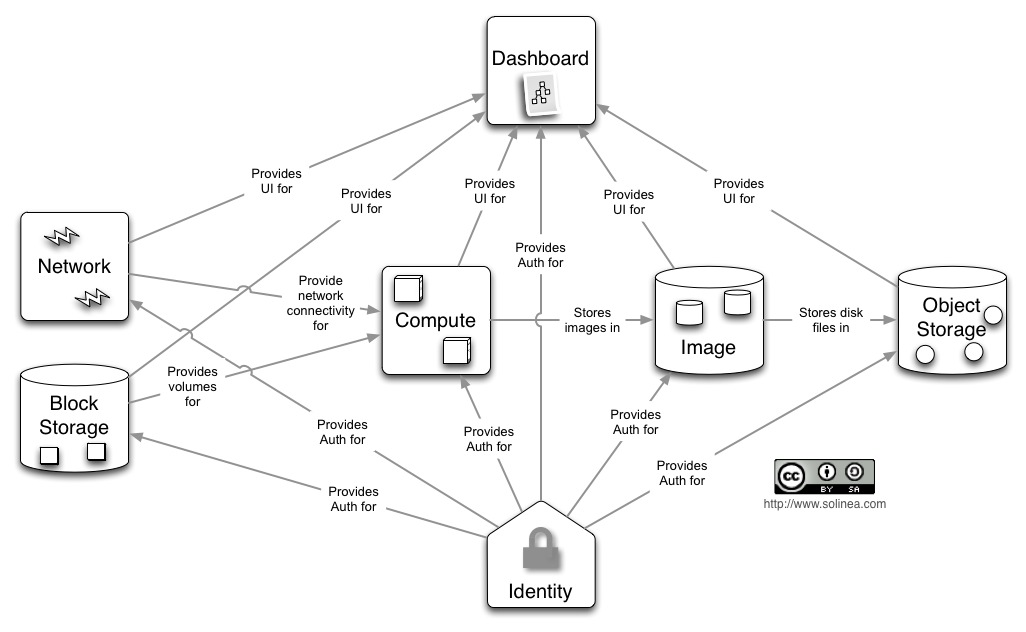
\includegraphics[width=0.85\textwidth]{openstack-arch}
    \caption{OpenStack核心组建的关系。源:OpenStack官方文档}
  \label{fig:openstack-arch}
\end{figure}
OpenStack跟AWS的架构很类似,分开计算,存储,网络和其他服务到不同的独立的组建。
在图\ref{fig:openstack-arch}可以看到OpenStack的核心组件和组件之间的关系。
OpenStack的Identity(Keystone)服务提供租户和权力管理功能,所有组件以来
Identity服务验证API请求是否有认证和权限。Compute(Nova)服务通过
虚拟化或裸服务器提供计算资源。Networking(Neutron)服务给Compute服务
提供网络资源的服务。Block Storage(Cinder)服务提供给Compute服务
块存储,块存储可以理解为虚拟硬盘服务。Image(Glance)服务保存
Compute服务的镜像,比如操作系统镜像或者用户传上的应用镜像。
Object Storage(Swift)是OpenStack的对象存储,保存任何文件,
Image服务可以配成用对象存储保存镜像的文件。Dashboard(Horizon)
是为所有组建提供Web界面,调用各个组建的RESTful API。了解到核心组建与
关系后,介绍计算,网络和存储组件的详细功能和实现方法。

\begin{wrapfigure}{r}{0.40\textwidth}
  \centering
    \includegraphics[width=0.39\textwidth]{openstack-comp-arch}
    \caption{OpenStack组建通用架构}
  \label{fig:openstack-comp-arch}
\end{wrapfigure}
OpenStack的每个组建都遵循统一个架构。在图\ref{fig:openstack-comp-arch}可以看到通用的架构,
每个组建有一个API层,负责提供对外的基于HTTP的RESTful API服务。如果API请求需要额外
处理比如创建虚拟机,API层会传信息到Message Queue,让任一个代理服务接受信息并且处理。
所有过程中需要,保存,更新或者删除持久的数据用到数据库。大部分组建也有一个Scheduler,
负责调度资源,比如选最合适创建虚拟机的hypervisor。API层,Agents和Scheduler都可以
横向扩展。

Compute是OpenStack的计算资源服务。Compute自己不包含虚拟化的软件,但是
它通过驱动方式抽象出来服务器资源。Compute目前支持的驱动包括Baremetal,KVM,Xen,
Hyper-V,LXC,VMWare vSphere。Compute的KVM虚拟化驱动是在OpenStack社区测试的最好和最受欢迎的驱动。
在2016的用户调查总计95\%的部署用KVM作为计算服务的技术选择。

Networking是OpenStack的网络资源服务。Networking服务抽象出来网络资源,让OpenStack运营商选不同的
网络技术实现Networking的服务。Networking是一个虚拟网络服务提供API让用户自己定义网络拓扑和管理IP地址,
另外也提供路由器,负载均衡和其他3层以上的网络服务。Compute使用Networking的服务提供给服务器网络链接。
Networking支持用OpenvSwitch,Linux Bridge和多个SDN厂家的技术。在2016的用户调查总计60\%的部署
用开源的OpenvSwitch作为Neutron的驱动。OpenvSwtich也是OpenStack社区官方推荐和支持度最高的驱动。

Block Storage是OpenStack的块存储服务。Block Storage服务抽象出来块存储的资源,OpenStack运营商可以选
不同的Cinder驱动的技术实现块存储。用户可以通过Block Storage的API,创建和管理块设备。一个块设备可以
理解为一个硬盘,硬盘可以从服务器拿走,插到其他服务器,通过Block Storage API一样可以操作块设备。
Block Storage支持的驱动包含主流的商业NAS/SAN存储和开源的分布式存储。在2016年用户调查总计,Ceph的开源分布式
排名第一,57\%部署使用Ceph作为Block Storage的后端存储。

Object Storage是OpenStack的对象存储服务。Object Storage是一个完全独立的组建,用户可以直接用对象存储保存
文件。用到的场景包含备份数据,大数据存储,应用数据(CSS,JS,图片等等)。



\section{自动部署与配置管理现况}
\label{subsec:automated_deployment}
随着DevOps文化的发展,强调开发者(Dev)和运维人员(Ops)的沟通和合作达到
同一目标,更快速,可靠,稳定发布和运营高质量的软件。达到目标通过自动化
软件的开发,测试,部署和运维的流程,促进流程更可靠和频繁被执行。
本章介绍DevOps常用的自动部署与配置管理工具,自动化运维和部署的流程。

如果没有自动化部署和配置,就造成可能在测试的时候部署与配置跟生产不一致,
自动化了部署与配置后,可以一样部署在测试生产,也可以避免人为故障。
在Linux最简单的方法自动化配置与安装是写Bash脚本,执行一系列的Linux命令。
用Bash脚本很有限制,很难做成幂等的脚本,保证如果脚本被执行多次,
执行后的结果每次都一样。对于可靠,稳定性能一模一样重复一个部署的环境很重要。
另外用Bash脚本没有标准化,不同的人可能用完全不一样结构和写法。
专门配置管理工具解决Bash脚本的问题,提供一个标准化幂等的自动部署工具。
本章介绍Puppet和Ansible的开源配置管理软件。


\subsection{Puppet}
既然IT运维人员维护的系统越来越多,强调运维自动化的重要性。
手工当然无法扩展到大规模的集群。
理想是有一个自动化系统,大家都可以用,而不是限于内部使用
脚本。Puppet协助运维人员社区建立和共享成熟的工具,
避免重复大家解决同一问题。Puppet以两种方式达到,第一
Puppet提供一个框架简单化大部分运维人员的技术任务,第二
用Puppet定义的语言可以容易分享和维护。
Puppet是一个在2005年被Puppet Labs开发的,
幂等和跨操作系统平台配置管理系统。\cite{puppet_docs}

\begin{wrapfigure}{r}{0.40\textwidth}
  \centering
    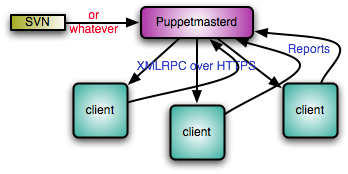
\includegraphics[width=0.38\textwidth]{puppet-master-slave}
    \caption{Puppet Master/Slave架构。\cite{puppet_docs}}
  \label{fig:puppet-master-slave}
\end{wrapfigure}
Puppet最常用的架构是一个Master/Slave架构。所有Slave定期(默认每30分钟)
从Master节点下载最新的配置,然后Slave保证本地配置跟从Master下载的配置是一致。
Slave执行完了配置更新,报给Master是否更新了配置还是原来的配置已经一致。

用Puppet自动化配置管理需要用Puppet基于Ruby定义的语言。Puppet语言的核心是
使用Resources,语言其他方面主要用处为了更灵活和方便的使用Resources。
一个Puppet Resource可能描述一个单独的系统包的状态或者文件的内容等等。
多个Resource可以被组织成一个Class,比如描述怎么配置整个应用,多个配置文件
,系统包等等。小的Class又可以被组织成一个更大的Class比如描述一个数据库服务角色。
Node(节点或者服务器)要分配多个角色需要分配它多个Class。指定哪些Class分配
到哪些Node叫Puppet的node classification。Puppet Modules(模块)是一种自我包含的包,
带运维人员写的Puppet的Resources, Classes和文件,促进容易共享和标准化的结构。

\subsection{Ansible}
\label{subsubsec:ansible}
Ansible跟Puppet一样是一个幂等的配置管理系统,简单化运维的自动化。跟Puppet主要区别在于架构和Ansible用YAML格式文件
定义系统配置的状态。Ansible的架构没有用Master/Slave的架构,Ansible没有用agents,这样被Ansible管的节点都
不需要装任何软件。Ansible通过高安全的SSH认真和访问被管理的节点。

Ansible通过自带modules抽象常用的资源比如装系统包。
Modules是在管理的节点被执行的部分,比如Ansible的apt module管理Debian/Ubuntu的包,用户可以通过apt模块指定
哪些包得装上哪些包不能装上。除了Ansible自带的modules用户也可以加自己的module。

Role是Ansible定义的目录结构,role目录下有tasks, handlers, templates, files, vars, defaults。Roles的
tasks,handlers,vars,defaults目录下得有一个main.yaml文件。tasks描述需要执行的modules和它们参数。handlers
描述发生时间可以被执行的任务,跟tasks很类似也是说明执行哪些modules和它们参数。
templates目录下保存所有模板化的文件,比如可以提供参数的配置文件。Files目录下保存
所有静态的文件,比如一些没有任何可调参数的配置文件。vars和defaults目录下的文件描述
role可调的参数,用role的用户可以通过role暴露的参数定定制适合自己的需求。

Ansible可以同时管理不同的基础设施环境。它通过inventory描述所有被管理的节点,
执行ansible可以制定需要用哪个inventory文件部署。另外也支持从基础设施云平台
动态的获取所有节点用作inventory。inventory文件用ini格式,每个section表示一个
server group(节点组),section下每行表示一个被管理的节点。

Ansible的playbook分配roles(角色)到在inventory里定义的节点组。用YAML格式描述
每个服务器得装那些软件,服务和配置。

%TODO: If time left provide a simple example



